\documentclass[a4paper,12pt,hidelinks]{report}

%%Pacchetti utili anche se non necessari

\usepackage{amsfonts}
\usepackage{amsmath}
\usepackage{latexsym}
\usepackage{tabularx}
\usepackage[italian]{babel}
\usepackage[bookmarks=true]{hyperref}
\usepackage{url}
% \usepackage{subfigure}
\usepackage{epstopdf}
\usepackage[utf8]{inputenc}
% \usepackage[utf8x]{inputenc}
\usepackage{listings}
\usepackage{graphicx}
\usepackage{color}

\usepackage{amsmath}


%-------------------------------------------

% \title{Progettazione sito web\\ ''B\&B La Vecchia Posta''}
% \author{Daniele Di Pompeo \\mat. 226766}
% \annoaccademico{2013-2014}
\begin{document}
  \begin{titlepage}
    \begin{center}
    % Upper part of the page
      
\includegraphics[width=0.5\textwidth,keepaspectratio=true]{../img/logo}\\[1cm]    
      \textsc{\LARGE Verifiche stile}\\[0.6cm]
      \textsc{\LARGE  progetto del sito:\\[0.5cm] ``B\&B La Vecchia Posta''}\\ [2.0cm]

    % Author and supervisor
      \begin{minipage}{0.8\textwidth}
	\begin{flushleft} \large
	  \emph{Autore:} Daniele Di Pompeo \\[0.5cm]
	  \emph{Versione documento: 1.0}\\[0.5cm]
	  \emph{Data emissione del documento: \today}\\[0.5cm]
	\end{flushleft}
      \end{minipage}
    \end{center}
  \end{titlepage}

% \tableofcontents
 
\begin{abstract}
In questo documento verranno analizzate e riportate le convalide alle scelte progettuali di visual design prese per il sito web \url{www.vecchiaposta.it}.
\\Un prima parte descriverà le scelte relative al comporto grafico, nella seconda parte invece si analizzerà il comportamento del sito web attraverso la 
\textit{cross-browser compatibility}.
\\In ultimo saranno mostrate le regole di accesibilità che il sito web garantisce.
\end{abstract}

\section*{Qualità della grafica}
Per valutare gli aspetti grafici si sono seguite le linee guide più classiche.

\begin{itemize}
 \item Gli oggetti cliccabili risultano essere tutti distinguibili grazie all'utilizzo di effetti di transizione grafica in alcuni casi e utilizzo di colori differenti in altri,
 con attenzione all'utilizzo del cursore ``pointer'' del mouse.
 \item Le varie sezioni del sito risultano essere identificabili grazie ad un effetto grafico sugli elementi del menu (aumento del weight del font). 
 \item Le varie sezioni del sito mantengono la stessa disposizione degli elementi non causando ``labirintite'' all'utente.
 \item I risultati ottenuti per il download dell'homepage si possono considerare accettabili. Si è eseguito un test utilizzando il servizio on-line offerto da \url{tools.pingdom.com/}
 di cui si riporta un screenshot.
 \begin{figure}[h!]%
    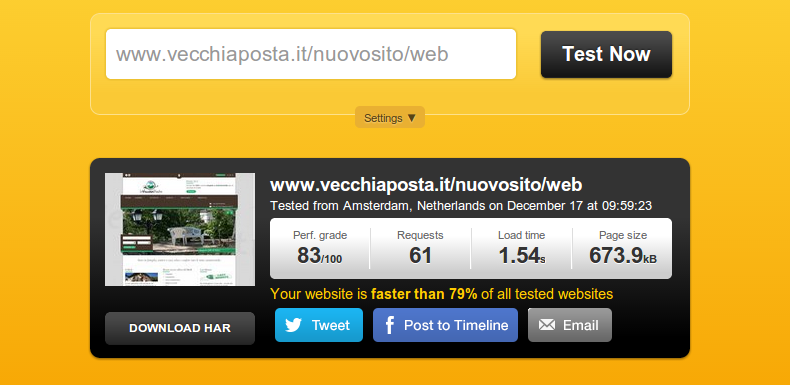
\includegraphics[width=0.8\textwidth,keepaspectratio=true]{../img/verificaAccessibilita}
    \centering
    \caption{Velocità di caricamento del DOM}%
    \label{fig:velAccesso}%
\end{figure}

\end{itemize}
 
\newpage
\section*{Presentazione della pagina}
Alle due risoluzioni, 1200px e 1024px, prese come risoluzioni base per lo sviluppo del sito web \url{www.vecchiaposta.it} non risultano essere presenti 
scroll orizzontali ma solamente scroll verticali. 
\par Le due risoluzioni risultano essere, da studi statistici del consorzio W3C sull'accessibilità del web, le due soluzioni maggiormente utilizzate nel comparto desktop. 

\newpage
\section*{Indipendenza tra browser}
Il sito web garantisce la \textit{cross-browser compatibility} rimanendo utilizzabile al 100\% anche tramite l'utilizzo di differenti browser.
In particolare l'intero progetto è stato sviluppato in ambiente linux su browser chrome, ma sono stati eseguiti test anche di compatibilità con
il browser Firefox, Opera ed Internet Explorer. L'unico browser non testato al momento è Safari di Apple Inc.
Di seguito si riportano alcuni screenshot per testimoniare la cross-browser compatibility.

\begin{figure}[h!]%
    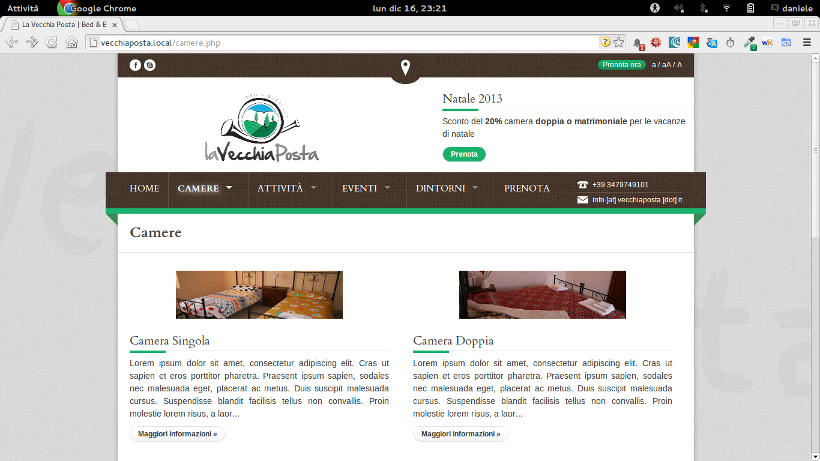
\includegraphics[width=0.8\textwidth,keepaspectratio=true]{../img/compChrome}
    \centering
    \caption{Compatibilità Chrome}%
    \label{fig:compChrome}%
\end{figure}

\begin{figure}[h!]%
    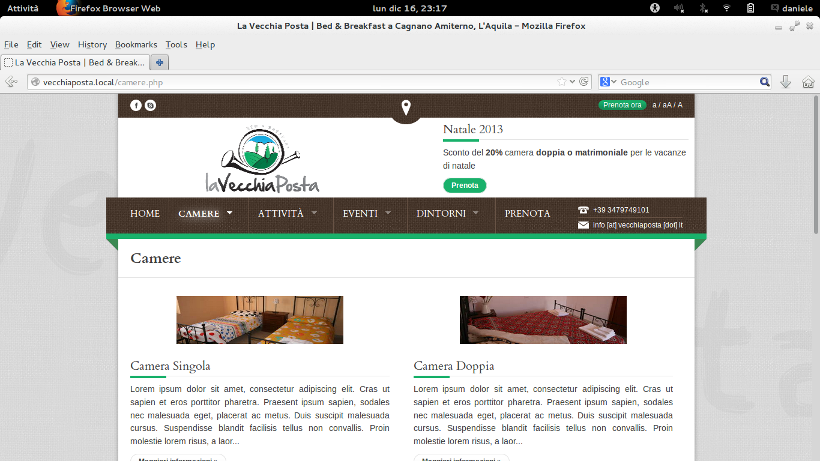
\includegraphics[width=0.8\textwidth,keepaspectratio=true]{../img/compFirefox}
    \centering
    \caption{Compatibilità Firefox}%
    \label{fig:compFirefox}%
\end{figure}

\begin{figure}[h!]%
    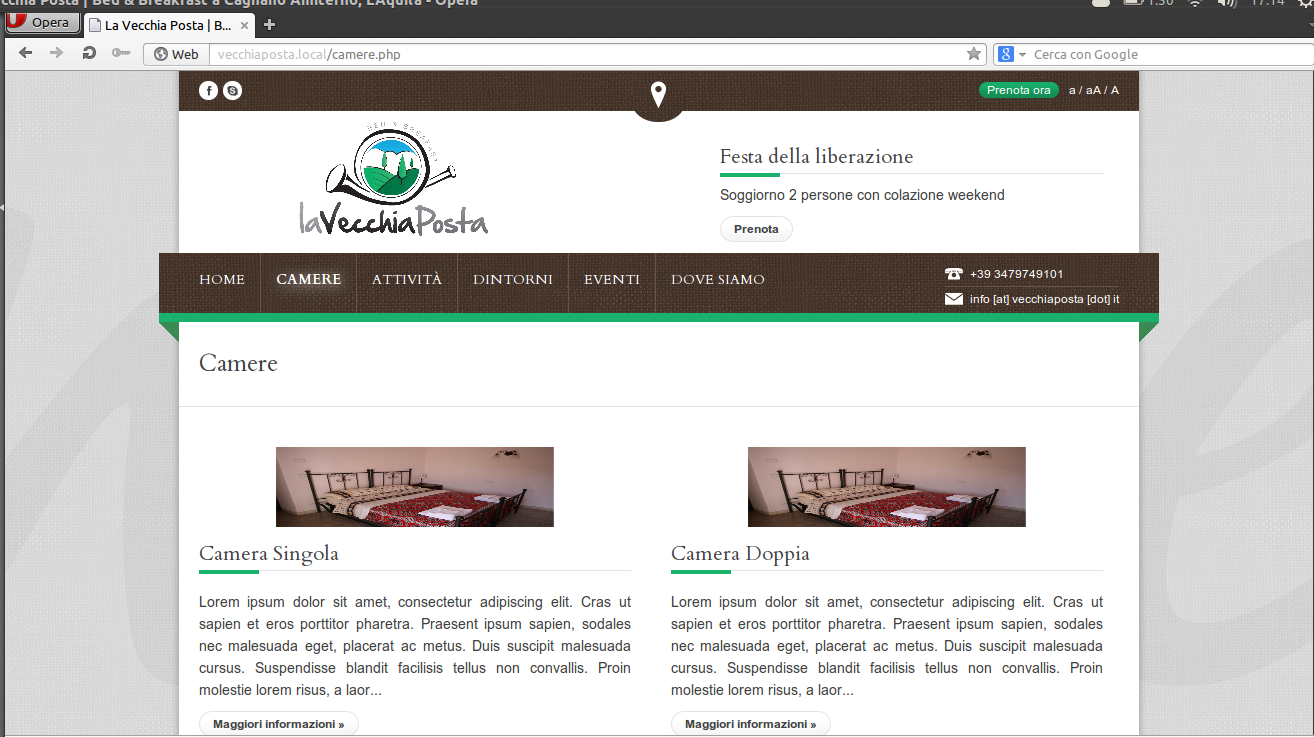
\includegraphics[width=0.8\textwidth,keepaspectratio=true]{../img/compOpera}
    \centering
    \caption{Compatibilità Opera}%
    \label{fig:compOpera}%
\end{figure}
\newpage
\begin{figure}[h!]%
    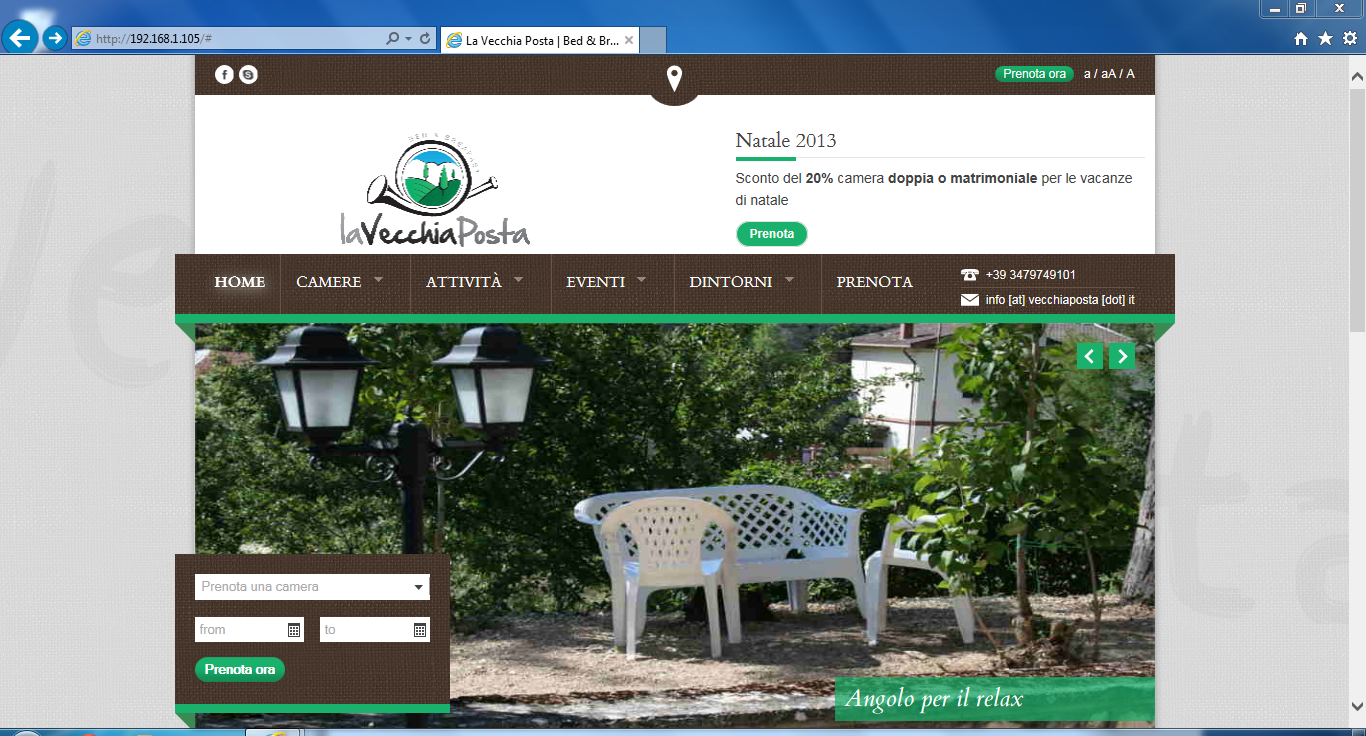
\includegraphics[width=0.8\textwidth,keepaspectratio=true]{../img/compIe10}
    \centering
    \caption{Compatibilità Internet Explorer 10}%
    \label{fig:compIe10}%
\end{figure}

\begin{figure}[h!]%
    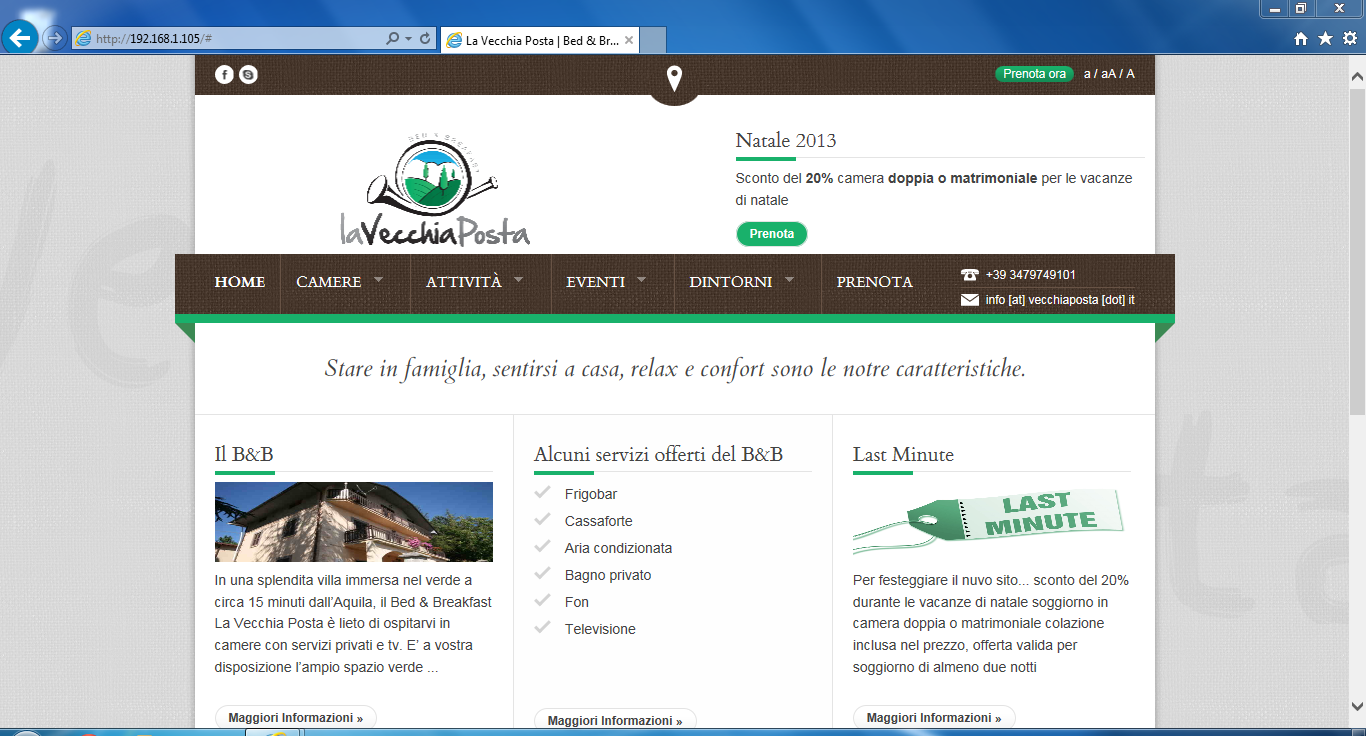
\includegraphics[width=0.8\textwidth,keepaspectratio=true]{../img/compIe9}
    \centering
    \caption{Compatibilità Internet Explorer 9}%
    \label{fig:compIe9}%
\end{figure}

\newpage
\section*{Utenti disabili}
Per quanto riguarda l'attenzione all'utilizzo dell'applicazione da utenti diversamente abili si è posta l'attenzione al disfunzionalità del daltonismo, simulandone l'utilizzo 
tramite servizi offerti online. Si riporta uno screenshot di esempio.

\begin{figure}[h!]%
    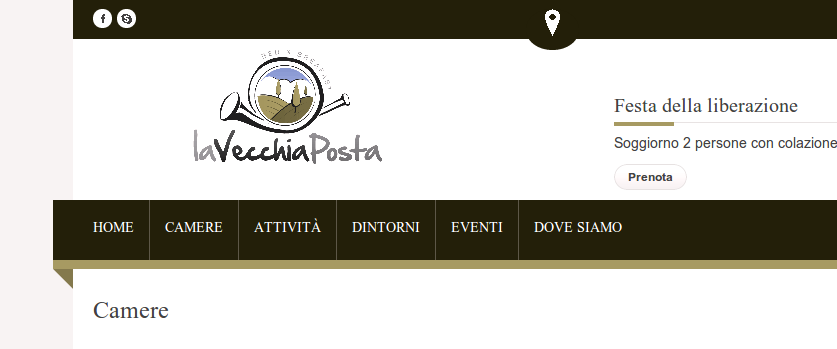
\includegraphics[width=0.9\textwidth,keepaspectratio=true]{../img/daltonismo}
    \centering
    \caption{Distorbo Protanopia}%
    \label{fig:daltonismo}%
\end{figure}
\par Non è stato l'unico test eseguito per testare la completa accessibilità dell'applicazione da utenti diversamente abili. 
Un altro test importante è stato testare l'applicazione tramite un browser testuale, nel nostro caso si è utilizzato Lynx disponibile per linux. 
L'utilizzo di un browser testuale aiuta ad individuare eventuali dimenticanze nel campo alt per le immagini ed evidenzia il corretto 
sviluppo dell'applicazione secondo le regole dei motori di ricerca che utilizzano software simili per i loro robots.

\begin{figure}[h!]%
    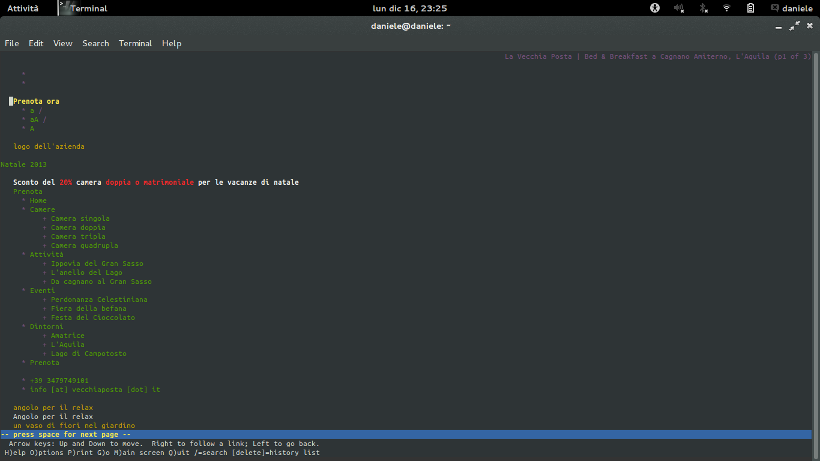
\includegraphics[width=0.9\textwidth,keepaspectratio=true]{../img/lynx}
    \centering
    \caption{Lynx scansione dell'applicazione}%
    \label{fig:lynx}%
\end{figure}

\newpage
\par Un ulteriore test per il check sull'accessibilità del sito è stato disabilitare il caricamento delle immagini e del javascript. Il risultato finale risulta essere non del 
tutto ottimale ma resta comunque accettabile. Si riporta di seguito uno screenshot del test. Si fa presente che al momento del test il browser chrome risulta avere un bug 
noto sul comportamento del campo alternativo alle immagini, si spera che in versioni successive ciò sarà risolto.
\begin{figure}[h!]%
    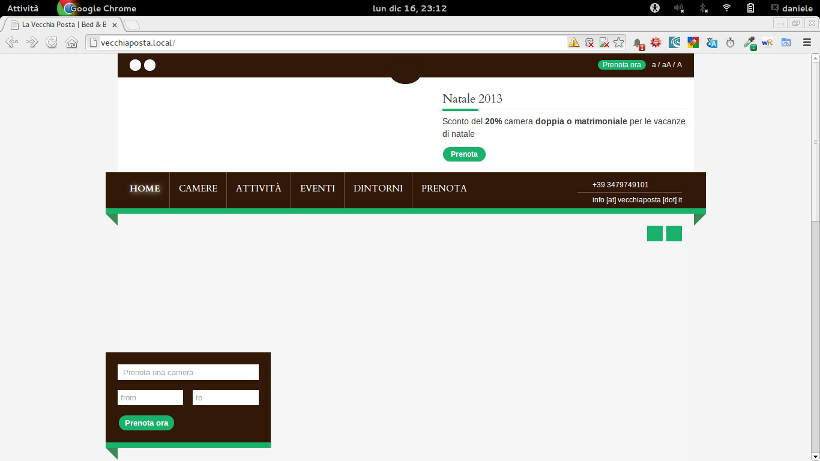
\includegraphics[width=0.9\textwidth,keepaspectratio=true]{../img/noJsNoImg}
    \centering
    \caption{Applicazione con Immagini e JavaScript bloccati}%
    \label{fig:noJsNoImg}%
\end{figure}

\newpage
\par Per garantire l'usabilità del sito web agli utenti ipovedenti si è implementata la funzionalità di controllo sulla dimensione del font della pagina.
In particolare si è garantito all'utente di modificare la dimensione del carattere del testo descrittivo le varie sezioni. 
\\Questo per non incappare in una modifica del layout di alcuni componenti, come la barra di navigazione
principale, per la quale si è utilizzato un carattere più grande rispetto al carattere base.
\par Si sono eseguiti anche alcuni test relativi alla luminosità del sito web. Questo per garantire la corretta visualizzazionde delle pagine e per permettere una facile lettura dei
contenuti.
\\Per il test della luminostità abbiamo utilizzato la seguente formula:

\[\frac{(red*299)+(green*587)+(bluee*114)}{1000} \geq {125}\]

tenstando la luminosità del menu, unico elemento ad avere del testo e un colore di sfondo differente dal bianco, il risultato è stato ottimo:

\[ \frac{(49*299)+(24*587)+(7*114)}{1000} = 295 \]

Per testare la differenza tra il colore del testo e il colore dello sfondo si è eseguito il test rispettando l'equazione:


\[[max(red1,red2)-min(red1,red2)]+ \]
\[+[max(green1,green2)-min(green1,green2)]+ \] 
\[+[max(blue1,blue2)-min(blue1,blue2)] \geq{500}\]

ottenendo come risultato

\[[244-49]+[244-24]+[244-7]={652}\]


\end{document}          